\documentclass{beamer}

\usepackage{beamerthemesplit}
\usepackage{amsfonts}

% Prepara o uso da lingua portuguesa
\usepackage{ucs}
\usepackage[utf8]{inputenc}
\usepackage[brazil]{babel}

% Para incluir graficos.
\usepackage{graphicx}

\usepackage{listings}

% Escolhendo o tema
\usetheme{Frankfurt}

% Arquivo dados.txt contém dados de título, autor etc.
\title[Segurança MQTT]{Segurança em MQTT} 
\author[A.C. André Luiz]{André Luiz Almeida Cardoso \\ Orientado por: Dr. Francisco José da Silva e Silva} 
\date{Setembro de 2019}
\institute[LSDi-UFMA]{Laboratório de Sistemas Distribuídos Inteligentes (LSDi)\\Universidade Federal do Maranhão (UFMA)\\\url{http://www.lsdi.ufma.br}}

\logo{
\includegraphics[width=2cm]{figuras/lsdi_ufma.png}} 


% Arquivo def.tex contém configurações dos pacotes em geral como o listings
\addtobeamertemplate{navigation symbols}{}{%
    \usebeamerfont{footline}%
    \usebeamercolor[fg]{footline}%
    \hspace{1em}%
    \insertframenumber/\inserttotalframenumber
}

%\usepackage[table,xcdraw]{xcolor}


\definecolor{verde}{rgb}{0.25,0.5,0.35}
\definecolor{jpurple}{rgb}{0.5,0,0.35}
\definecolor{darkgreen}{rgb}{0.0, 0.2, 0.13}

\newcommand{\estiloJava}{
\lstset{
    language=Java,
    basicstyle=\ttfamily\small,
    keywordstyle=\color{jpurple}\bfseries,
    stringstyle=\color{red},
    commentstyle=\color{verde},
    morecomment=[s][\color{blue}]{/**}{*/},
    extendedchars=true,
    showspaces=false,
    showstringspaces=false,
    numbers=left,
    numberstyle=\tiny,
    breaklines=true,
    backgroundcolor=\color{cyan!10},
    breakautoindent=true,
    captionpos=b,
    xleftmargin=0pt,
    tabsize=2
}} 
\bibliographystyle{apalike}


\begin{document}

\frame{\titlepage}
% ----------------------------------------------------------------
\section[Sumário]{}

\frame{
\frametitle{Sumário Normal}
\tableofcontents
}
% ----------------------------------------------------------------
\AtBeginSection[]
{
\begin{frame}
\frametitle{Sumário}
\tableofcontents[currentsection]
\end{frame}
}

\section{Conceitos Iniciais}

% ----------------------------------------------------------------
%
%\frame{
%	\frametitle{Infraestrutura M-Hub/CDDL}
%\begin{figure}[!ht]
%	\begin{center}
%		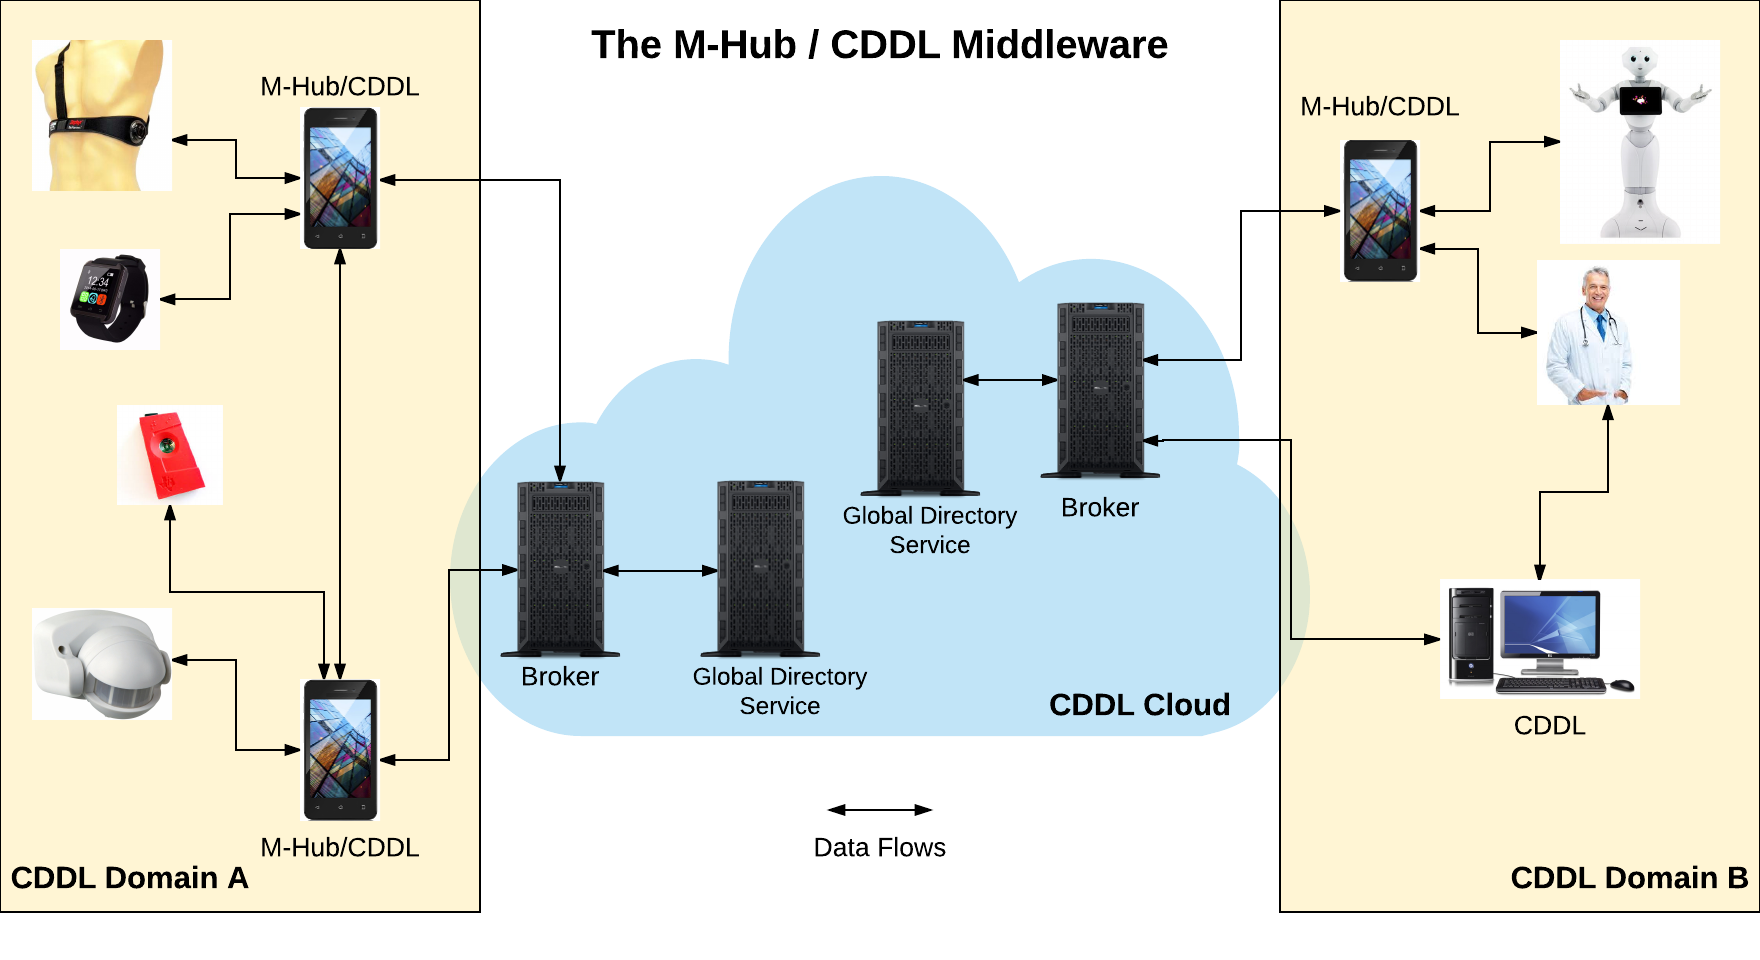
\includegraphics[scale=0.18]{figuras/cddl-domains.png}
%		\label{fig:cddl-domains}
%	\end{center}
%\end{figure}

%}

\frame {
	\frametitle{MQTT - Message Queuing Telemetry Transport [ibm]}
	\begin{itemize}
		\item Histórico
		\begin{itemize}
			\item O MQTT foi criado pela IBM no fim da década de 1990;
			\item Finalidade de vincular sensores em pipelines de petróleo a
			satélites;
			\item Assíncrono;
			\item Utiliza o modelo Publish/Subscribe;		
		\end{itemize}
		\bigskip
		\item Por que usar MQTT em IoT?
		\begin{itemize}
			\item Leve;
			\item Flexivel;
			\item Permite uso de dispositivos com capacidade de memoria e processamento limitados;
			\item Escalável;
			
		\end{itemize}
		\bigskip
		
	\end{itemize}
	% Vc pode usar \smallskip também...
}

\frame {
	\frametitle{MQTT - Funcionamento}
			\begin{itemize}
		\item CONNECT message
		\item PUB: /sensor/data
		\item SUB: /sensor/data
	\end{itemize}
	
	\begin{figure}[!ht]
		\begin{center}
			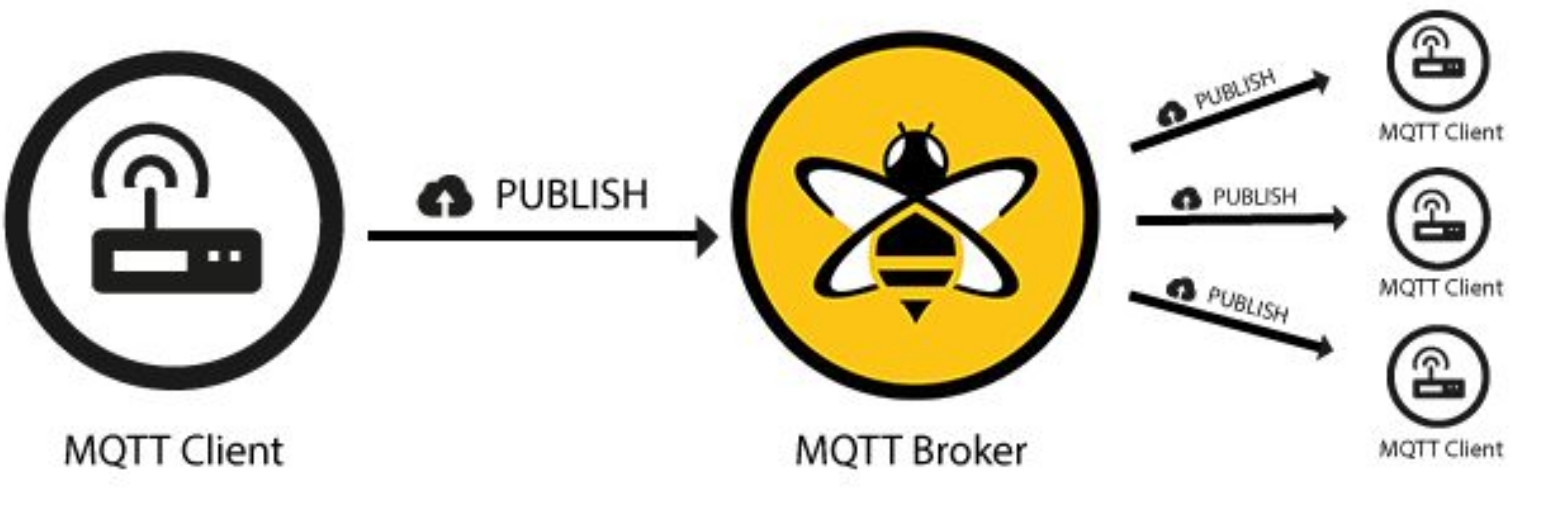
\includegraphics[scale=0.18]{figuras/mqtt.png}
			\caption{MQTT example. [hiveMQ]}
			\label{fig:mqtt}
		\end{center}
	\end{figure}
}


\frame {
\frametitle{Segurança - Conceitos Iniciais}


\begin{columns}
	\begin{column}{0.48\textwidth}
		
		\begin{itemize}
			\item Confiabilidade:	
			\begin{itemize}
				\item Confidencialidade;
				\item Integridade;									
			\end{itemize}	
			
		\end{itemize}
	
		
	\end{column}
		\begin{column}{0.48\textwidth}
			
				\begin{itemize}
				\item Criptografia;
				\item Autenticação;
				\item Autorização;
				\item Auditoria;
			\end{itemize}

		 
	 
		\end{column}
\end{columns}

% Vc pode usar \smallskip também...
}


\frame {
\frametitle{Segurança - Criptografia Simetrica [tanembaum]}


\begin{itemize}
	\item Sistemas de chaves compartilhadas;
	\item Mesma chave é usada para cifrar e decifrar;
	\item Chave deve ser mantida em segredo;
	\item Limitações: escalabilidade;
	\item Algoritmos conhecidos: DES, DES triplo;
\end{itemize}
% Vc pode usar \smallskip também...
}


\frame {
	\frametitle{Segurança - Criptografia Assimétrica [tanembaum]}
	
	
	\begin{itemize}
		\item Sistema de chaves publicas;
		\item Chaves diferentes para cifrar e decifrar;
		\item Chave publica para cifrar;
		\item Chave privada para decifrar;
	
	\end{itemize}
	% Vc pode usar \smallskip também...
}

\frame {
	\frametitle{Segurança - Assinatura digital [tanembaum]}
	
	
	\begin{itemize}
		\item Forma de garantir a integridade e não repudio;
		\item Usa-se funções hash (MD5,SHA,etc);
		
	\end{itemize}
	% Vc pode usar \smallskip também...
}



\frame {
	\frametitle{Segurança - Certificado digital [tanembaum]}
	
	\begin{figure}[!ht]
		\begin{center}
			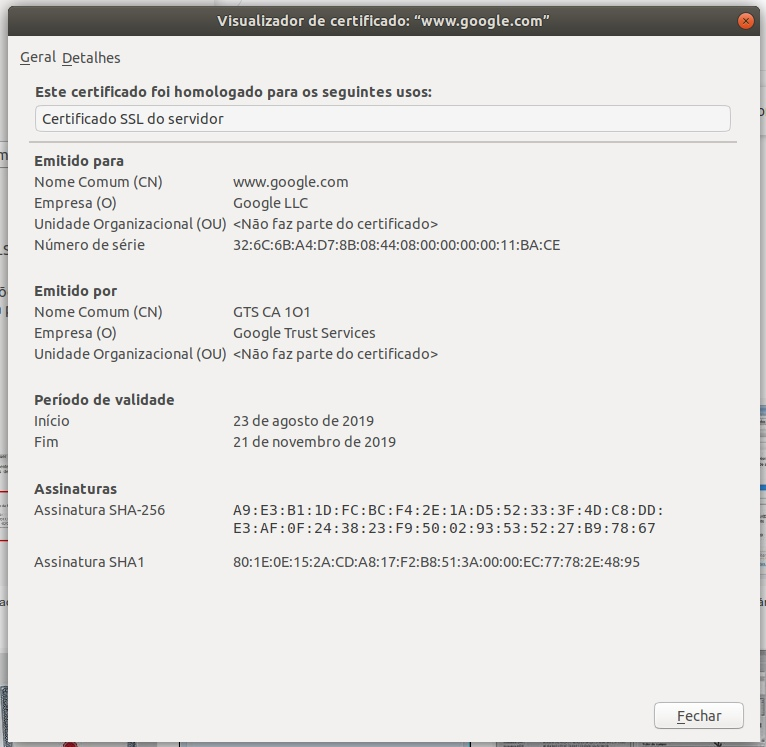
\includegraphics[scale=0.2]{figuras/cert.jpg}
			\caption{Certificado Digital: google.com}
			\label{fig:mqtt}
		\end{center}
	\end{figure}
	
	% Vc pode usar \smallskip também...
}
\frame {
	\frametitle{Segurança - Autoridade Certificadora}
	
	\begin{figure}[!ht]
		\begin{center}
			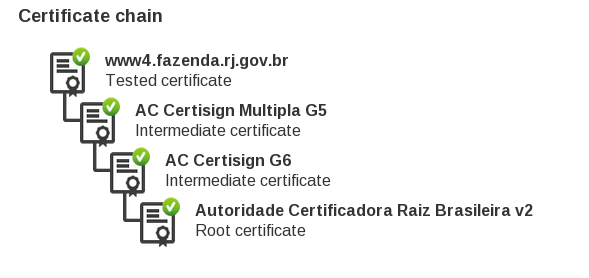
\includegraphics[scale=0.4]{figuras/cachain.png}
			\caption{Fonte: \url{https://bit.ly/2kdvRkW}}
			\label{fig:mqtt}
		\end{center}
	\end{figure}
	
	% Vc pode usar \smallskip também...
}


\section{Segurança no MQTT}

\frame{
\frametitle{Segurança no MQTT - Nível de Rede}
\begin{itemize}
	\item Utilizar uma rede fisicamente segura:

	\begin{itemize}
		\item Acesso fisico ao servidor;
		\item Controle das chaves; 
		\item Utilizar racks com cadeados;
		\item Trancar a sala do computador;
		\bigskip
	\end{itemize}
	\item VPN para comunicação entre clientes e brokers:
	
	\begin{itemize}
		\item Adequado para aplicações gateway;

	\end{itemize}
\end{itemize}
}

\frame{
	\frametitle{Segurança no MQTT - Nível de Transporte}
	\begin{itemize}
		
		\item Confidencialidade;
		\bigskip
		\item Integridade;
		\bigskip
		\item Autenticação;
		\bigskip
		\item Autorização;
		\bigskip
		\item Auditoria;
	\end{itemize}
}



\frame{
	\frametitle{Segurança no MQTT - Nível de Transporte - TLS/SSL}
	\begin{definition}
		At the core, TLS and SSL are cryptographic protocols which use a handshake mechanism to negotiate various parameters to create a secure connection between the client and the server. [1]
	\end{definition}
	\begin{itemize}
		\item MQTT já possui suporte ao TLS, ao utiliza-lo, obtemos:
		\begin{itemize}
			\item Confidencialidade;
			\item Integridade;
		\end{itemize}
		\item Autenticação:
		\begin{itemize}
			\item TLS via certificado (cliente e servidor);
			\item Broker via usuario e senha;
		\end{itemize}
			\item Auditoria:
		\begin{itemize}
			\item Feita no broker via Logs;
			
		\end{itemize}
		
	\end{itemize}
}



\frame{
\frametitle{Segurança no MQTT - Nível de Transporte - TLS/SSL}
\begin{figure}[!ht]
		\begin{center}
			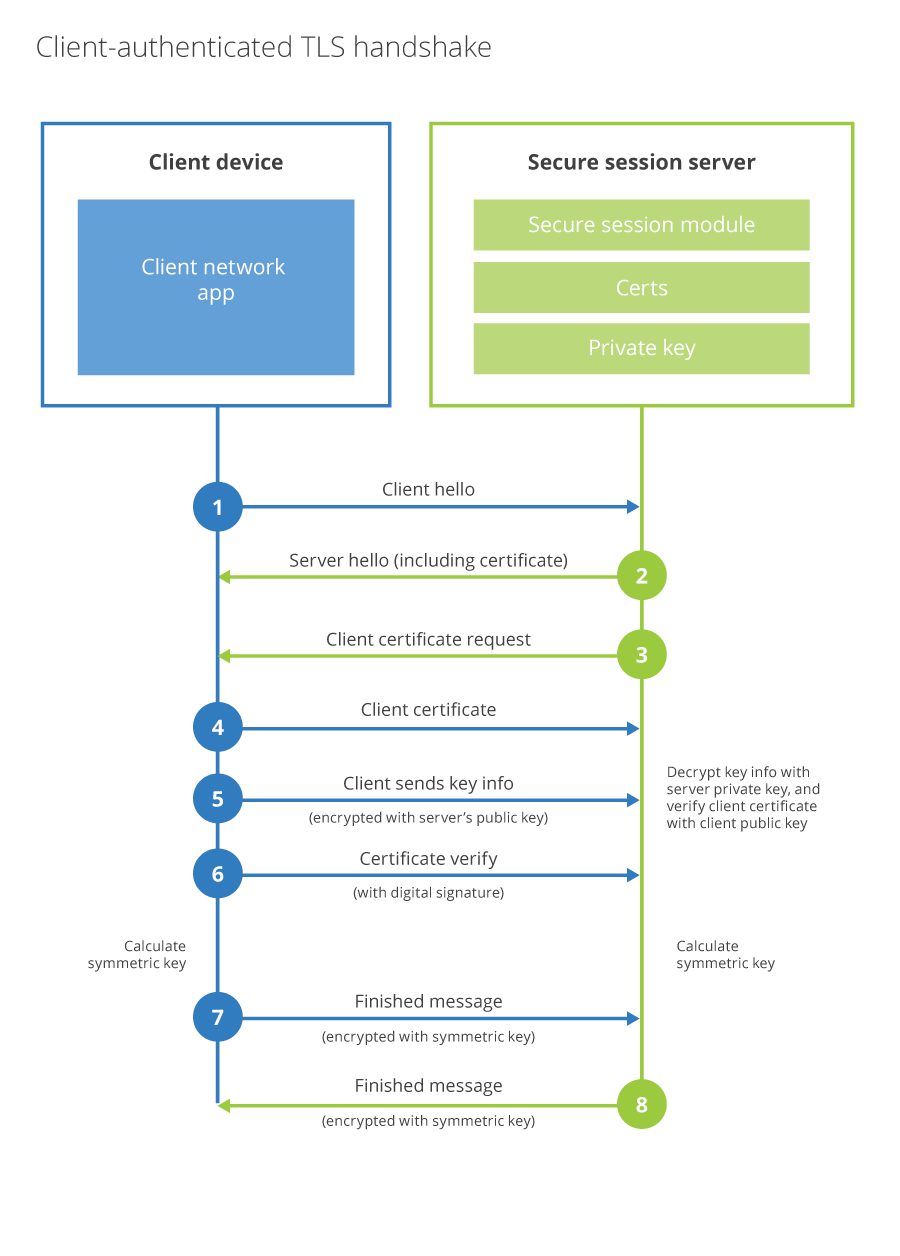
\includegraphics[scale=0.18]{figuras/tls2.png}
			\label{fig:cddl-arch}
		\end{center}
	\end{figure}
	
}


\frame{
	\frametitle{Segurança no MQTT - Nível de Transporte - Autenticação}
\begin{itemize}
	\item CONNECT message:
	\begin{itemize}
		\item Autenticação via usuario e senha no Broker MQTT
	\end{itemize}	
\end{itemize}
\begin{figure}[!ht]
	\begin{center}
		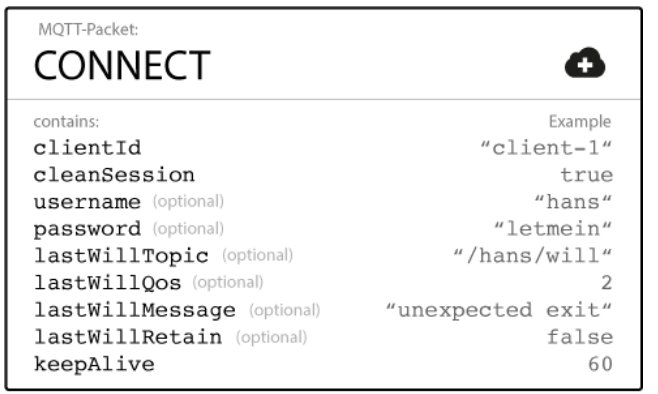
\includegraphics[scale=0.3]{figuras/auth.jpg}
		\label{fig:auth}
	\end{center}
\end{figure}

}

\frame{
	\frametitle{Segurança no MQTT - Nível de Aplicação}
	\begin{itemize}
		\item Autenticação
		\item Criptografia simétrica
			
	\end{itemize}
	
	
}


\section{Segurança - Mosquitto}

\frame{
\frametitle{Configurando Broker - Mosquitto}
\begin{itemize}
	\item https://mosquitto.org/download/
	\item TLS;
	\item Autenticação cliente e servidor via certificado;
	\item Autenticação cliente via usuário e senha;
	\item Autorização via ACL no broker;
	
\end{itemize}
}
\frame{
	\frametitle{Configurando Broker - Mosquitto - TLS}
	
	\begin{columns}
		\begin{column}{0.4\textwidth}
			
			\begin{itemize}
				\item[] Requisitos do Broker:
				\begin{itemize}
					\item Certificado da CA;
					\item Certificado do servidor; 
					\item Chave privada;	 
				\end{itemize}
				
			\end{itemize}
			\begin{itemize}
				\item[] Requisitos do Cliente:
				\begin{itemize}
					\item Certificado da CA;	 
				\end{itemize}
				
			\end{itemize}
			
		\end{column}
		\begin{column}{0.5\textwidth}
		
		\begin{enumerate}
			\item Par de chaves para CA;
			\item Certificado da CA;
			\item Chaves para o broker;
			\item certificado do broker;
			\item Assinar o certificado do broker com a CA;
		\end{enumerate}
			
		\end{column}
	\end{columns}
	
}

\frame{
	\frametitle{Configurando Broker - Mosquitto - TLS}
	

	
	\begin{enumerate}
		\item[] Gerando arquivos necessários:
		\begin{itemize}
			\item \$ openssl genrsa -des3 -out ca.key 2048
			\item  \$ openssl req -new -x509 -days 1826 -key ca.key -out ca.crt
			\item \$ openssl genrsa -out server.key 2048
			\item \$ openssl req -new -out server.csr -key server.key
			\item \$ openssl x509 -req -in server.csr -CA ca.crt -CAkey ca.key -CAcreateserial -out server.crt -days 360
		\end{itemize}	
		\item[] Output:
		\begin{itemize}
			\item \colorbox{yellow}{ca.crt}
			\item ca.key
			\item ca.srl
			\item server.csr
			\item \colorbox{yellow}{server.crt}
			\item \colorbox{yellow}{server.key}
			
		\end{itemize}
	\end{enumerate}
}

\frame{
	\frametitle{Configurando Broker - Mosquitto - TLS}
	
	
	Mova os arquivos para:
	\begin{itemize}
	
		\item[] /etc/mosquitto/certs:
		\begin{itemize}
		
			\item \colorbox{yellow}{server.crt}
			\item \colorbox{yellow}{server.key}
			
		\end{itemize}
		
		\item[] /etc/mosquitto/ca\_certificates
		\begin{itemize}
			\item \colorbox{yellow}{ca.crt}
		\end{itemize}		
		
	
	\end{itemize}

}


\frame{
	\frametitle{Configurando Broker - Mosquitto - TLS}
	
	
	\begin{itemize}
		\item Altere o arquivo de configuração;
		\item /etc/mosquitto/conf.d/\colorbox{yellow}{local.conf}		
		\begin{itemize}
			\bigskip
			\item[] port 8883 \bigskip
			
			\item[] allow\_anonymous true \bigskip
			
			\item[] password\_file /etc/mosquitto/passwordfile\bigskip
			\item[] cafile /etc/mosquitto/ca\_certificates/ca.crt\bigskip
			
			\item[] keyfile /etc/mosquitto/certs/server.key\bigskip
			
			\item[] certfile /etc/mosquitto/certs/server.crt\bigskip
			
			\item[] require\_certificate false\bigskip
			
			\item[] use\_identity\_as\_username false
			
		\end{itemize}
	\end{itemize}
		
}

\frame{
	\frametitle{Configurando Broker - Mosquitto - TLS}
	
	\begin{itemize}
		\item TLS já configurado;
		\item Apenas o cliente autentica o servidor;
		\item Cliente necessita do certificado da CA que assinou o certificado do broker;

		\item \$mosquitto -c /etc/mosquitto/conf.d/local.conf
		
		\item \text{\$mosquitto\_sub -p 8883 -h localhost -t /hello \texttt{-{}-}cafile ca.crt} 
		
		
		\item \$mosquitto\_pub -p 8883 -h localhost -t /hello -m "ola TLS" \texttt{-{}-}cafile ca.crt 
		
	\end{itemize}
}


\frame{
	\frametitle{Configurando Broker - Mosquitto - Autenticação}
	
	\begin{itemize}
		\item Autenticação via usuário e senha:
		\begin{itemize}
			\item[] allow\_anonymous false 
			\item[] password\_file /etc/mosquitto/passwordfile
		\end{itemize}
		\item passwordfile.txt\\
		\fbox{\begin{minipage}{15em}
				andre:changeme\\
				igor:123456\\
				pablo:654321
		\end{minipage}}	\bigskip
		\item \$mosquitto\_passwd -U passwordfile \\
			
		\fbox{\begin{minipage}{15em}
				andre:\$6\$Y97FBWT4pKzYH1Fv...
				igor:\$6\$3E5ZgxX6pwYPikJr...
				pablo:\$6\$O1+MiKq+BfhhMzJg...
		\end{minipage}}	
		
		
	\end{itemize}

}

\frame{
	\frametitle{Configurando Broker - Mosquitto - Autenticação}
	
	\begin{itemize}

		
		\item \$mosquitto -c /etc/mosquitto/conf.d/local.conf
		
		\item \text{\$mosquitto\_sub -p 8883 -h localhost -t /hello \texttt{-{}-}cafile ca.crt} -u andre -P "123456"
		
			
		\item \$mosquitto\_pub -p 8883 -h localhost -t /hello -m "ola TLS" \texttt{-{}-}cafile ca.crt -u andre -P "123456"
		
		
	\end{itemize}
}
\frame{
	\frametitle{Configurando Broker - Mosquitto - Autenticação}
	
	\begin{itemize}
		\item[] Autenticação via certificado do cliente;
		\begin{itemize}
			\item[] require\_certificates true 
			\item[] use\_identity\_as\_username false
			\item[] crlfile /path/to/crlfile
		\end{itemize}
		\item[] Criando o certificado do cliente:
		\begin{enumerate}
			\item Criar chave do cliente; 
			\item Criar o certificado do cliente usando a chave;
			\item Assinar o certificado do cliente com a mesma CA que assinou o servidor;
		\end{enumerate}
	
	\end{itemize}

}


\frame{
	\frametitle{Configurando Broker - Mosquitto - Autenticação}
	
	\begin{itemize}
		
		\item Criando o certificado do cliente:
		\begin{enumerate}
			\item  \$openssl genrsa -out client.key 2048
			\item  \$openssl req -new -out client.csr -key client.key
			\item  \$openssl x509 -req -in client.csr -CA ca.crt -CAkey ca.key -CAcreateserial -out client.crt -days 360
		\end{enumerate}
		\item Output:
		\begin{itemize}
			\item \colorbox{yellow}{client.key}
			\item client.csr
			\item \colorbox{yellow}{client.crt}
		\end{itemize}
	\end{itemize}
}


\frame{
	\frametitle{Configurando Broker - Mosquitto - Autenticação}
	
	\begin{itemize}
		\item[] Autenticação via certificado do cliente;

		
		\item \$mosquitto\_sub -p 8883 -h localhost -t /hello \texttt{-{}-}cafile ca.crt \texttt{-{}-}cert client.crt \texttt{-{}-}key client.key\bigskip
		
		\item \$mosquitto\_pub -p 8883 -h localhost -t /hello -m "olá tls" \texttt{-{}-}cafile ca.crt \texttt{-{}-}cert client.crt \texttt{-{}-}key client.key \bigskip
	
	\end{itemize}
}

\frame{
	\frametitle{Configurando Broker - ACL }
	
	\begin{itemize}
		\item acl\_file path/to/\colorbox{yellow}{acl.txt} \bigskip
		\begin{itemize}
			\item Afeta os clientes sem usuario:
			\begin{itemize}
				\item[] topic read /topic \bigskip
			\end{itemize}
			\item Afeta o username:
			\begin{itemize}
				\item[] user andre
				\item[] topic write /topic\bigskip
			\end{itemize}
		\item Afeta todos os clientes:
		\begin{itemize}
			\item[] pattern readwrite /topic/\%u/\# \bigskip
		\end{itemize}
		\end{itemize}
		
	\end{itemize}
}

\frame{
	\frametitle{Configurando Broker - CRL }
	\begin{enumerate}
		\item https://www.hivemq.com/mqtt-security-fundamentals/
		
	\end{enumerate}
}

\frame{
	\frametitle{Configurando Broker - Auditoria }
	\begin{itemize}
		\item Via logs no broker;
		\item Alterando arquivo de configurações:
		\begin{itemize}
			\item log\_type [debug, error, warning, notice, information, subscribe, unsubscribe, websockets, none, all.]
			\item log\_dest file /path/to/mosquitto.log
		\end{itemize}
		
	\end{itemize}
}


\section{Segurança - Moquette}
\frame{
	\frametitle{Configurando Broker - Moquette}
	\begin{enumerate}
		\item \url{https://github.com/moquette-io/moquette};
		\item Implementado em Java;
		\item Arquivos de configuração semelhantes ao Mosquitto;
		\item Possivel utilizar keystores;
		\item Fornece Interfaces para configurações customizadas;
	\end{enumerate}
}



\frame{
	\frametitle{Referências}
	\begin{enumerate}
		\item \url{https://www.hivemq.com/mqtt-security-fundamentals/}
		\item \url{https://github.com/moquette-io/moquette}
	\end{enumerate}
}

\end{document}

